\chapter{Opis projektnog zadatka}
		
		\textbf{\textit{Cilj projektnog zadatka}}\\
		
		\textit{Kako je zdravlje najvažnija stvar u ljudskome životu za normalnu funkcionalnost društva, došlo je vrijeme da stvari krenu na bolje i da se naše zdravstvo modernizira. Zdravstvo samo po sebi je ogroman sustav sa jako puno sudionika, bilo radnika ili pacijenata, stoga se na prvu čini jako teško riješiti problem ubrzanja naručivanja pregleda i poboljšanja korisničkih usluga u zdravtsvu. No, nakon sažimanja i kompresiranja problema u manje stavke, možemo sa sigurnošću reći da je problem rješiv i ostvariv. Cilj ovog projektnog zadatka je realizirati sustav planiranja zdravstvenih usluga i komunikacije s 
korisnicima koji bi omogućio učinkovite primarne, polikliničke i bolničke zdravstvene usluge u hrvatskom zdravstvu, lako dostupne svim građanima. U daljnjim točkama objasnit će se sva problematika i solucije projekta.
ogleda se u dva osnovna aspekta njegove realizacije. Sustav će biti realiziran korištenjem AngularJS frontend okvirom kao web aplikacija dostupna svim građanima Republike Hrvatske.  } \newline \newline
                \textbf{\textit{Funkcionalnosti aplikacije}}\\
            \newline
            \textit{}
            \textit{
            Korisnici aplikacije će biti pacijenti, liječnici, medicinske sestre i administratori. Osnovna funkcionalnost dostupna pacijentima je zakazivanje pregleda kod 
liječnika opće medicine te slanje podsjetnika za termine putem SMS poruka ili 
e-pošte. }	
		\textit{Za pomoć pogledati reference navedene u poglavlju „Popis literature“, a po potrebi konzultirati sadržaj na internetu koji nudi dobre smjernice u tom pogledu.}
       \newline
       \newline
            \textbf{\textit{Potencijalna korist projekta}}\\ 
            \newline
            \textit{Korist ovog projekta može se iskazati na više načina. Korisnost samog rada biti će na pomoć najprije djelatnicima hrvatskog zdravstva koji će biti odriješeni javljanja na telefon i odgovaranja na email poruke svojih pacijenata, već će biti u mogućnosti fokusirati se na svoj rad, a ne gubiti vrijeme na formalnosti. Naravno, ovaj sustav će biti jednako tako koristan i pacijentima koji neće morati pisati duge mailove i čekati nekoliko dana kako bi im se djelatnik javio na poziv. Dakle s obje strane imamo veliko poboljšanje. Sustav će omogućiti konstantnu mogućnost prijave pregleda kod željenog zdravstvenika, neovisno koji je dan u tjednu. Pacijenti će tako imati sigurniji život i puno će brže obavljati samo prijavu pregleda. }
             \newline
            \newline
            \textbf{\textit{Primjeri sličnih rješenja u stvarnosti}}\\ 
      
		
		\section{Primjeri u \LaTeX u}
		
		\textit{Ovo potpoglavlje izbrisati.}\\

		U nastavku se nalaze različiti primjeri kako koristiti osnovne funkcionalnosti \LaTeX a koje su potrebne za izradu dokumentacije. Za dodatnu pomoć obratiti se asistentu na projektu ili potražiti upute na sljedećim web sjedištima:
		\begin{itemize}
			\item Upute za izradu diplomskog rada u \LaTeX u - \url{https://www.fer.unizg.hr/_download/repository/LaTeX-upute.pdf}
			\item \LaTeX\ projekt - \url{https://www.latex-project.org/help/}
			\item StackExchange za Tex - \url{https://tex.stackexchange.com/}\\
		
		\end{itemize} 	


		
		\noindent \underbar{podcrtani tekst}, \textbf{podebljani tekst}, 	\textit{nagnuti tekst}\\
		\noindent \normalsize primjer \large primjer \Large primjer \LARGE {primjer} \huge {primjer} \Huge primjer \normalsize
				
		\begin{packed_item}
			
			\item  primjer
			\item  primjer
			\item  primjer
			\item[] \begin{packed_enum}
				\item primjer
				\item[] \begin{packed_enum}
					\item[1.a] primjer
					\item[b] primjer
				\end{packed_enum}
				\item primjer
			\end{packed_enum}
			
		\end{packed_item}
		
		\noindent primjer url-a: \url{https://www.fer.unizg.hr/predmet/proinz/projekt}
		
		\noindent posebni znakovi: \# \$ \% \& \{ \} \_ 
		$|$ $<$ $>$ 
		\^{} 
		\~{} 
		$\backslash$ 
		
		
		\begin{longtblr}[
			label=none,
			entry=none
			]{
				width = \textwidth,
				colspec={|X[8,l]|X[8, l]|X[16, l]|}, 
				rowhead = 1,
			} %definicija širine tablice, širine stupaca, poravnanje i broja redaka naslova tablice
			\hline \multicolumn{3}{|c|}{\textbf{naslov unutar tablice}}	 \\ \hline[3pt]
			\SetCell{LightGreen}IDKorisnik & INT	&  	Lorem ipsum dolor sit amet, consectetur adipiscing elit, sed do eiusmod  	\\ \hline
			korisnickoIme	& VARCHAR &   	\\ \hline 
			email & VARCHAR &   \\ \hline 
			ime & VARCHAR	&  		\\ \hline 
			\SetCell{LightBlue} primjer	& VARCHAR &   	\\ \hline 
		\end{longtblr}
		

		\begin{longtblr}[
				caption = {Naslov s referencom izvan tablice},
				entry = {Short Caption},
			]{
				width = \textwidth, 
				colspec = {|X[8,l]|X[8,l]|X[16,l]|}, 
				rowhead = 1,
			}
			\hline
			\SetCell{LightGreen}IDKorisnik & INT	&  	Lorem ipsum dolor sit amet, consectetur adipiscing elit, sed do eiusmod  	\\ \hline
			korisnickoIme	& VARCHAR &   	\\ \hline 
			email & VARCHAR &   \\ \hline 
			ime & VARCHAR	&  		\\ \hline 
			\SetCell{LightBlue} primjer	& VARCHAR &   	\\ \hline 
		\end{longtblr}
	


		
		
		%unos slike
		\begin{figure}[H]
			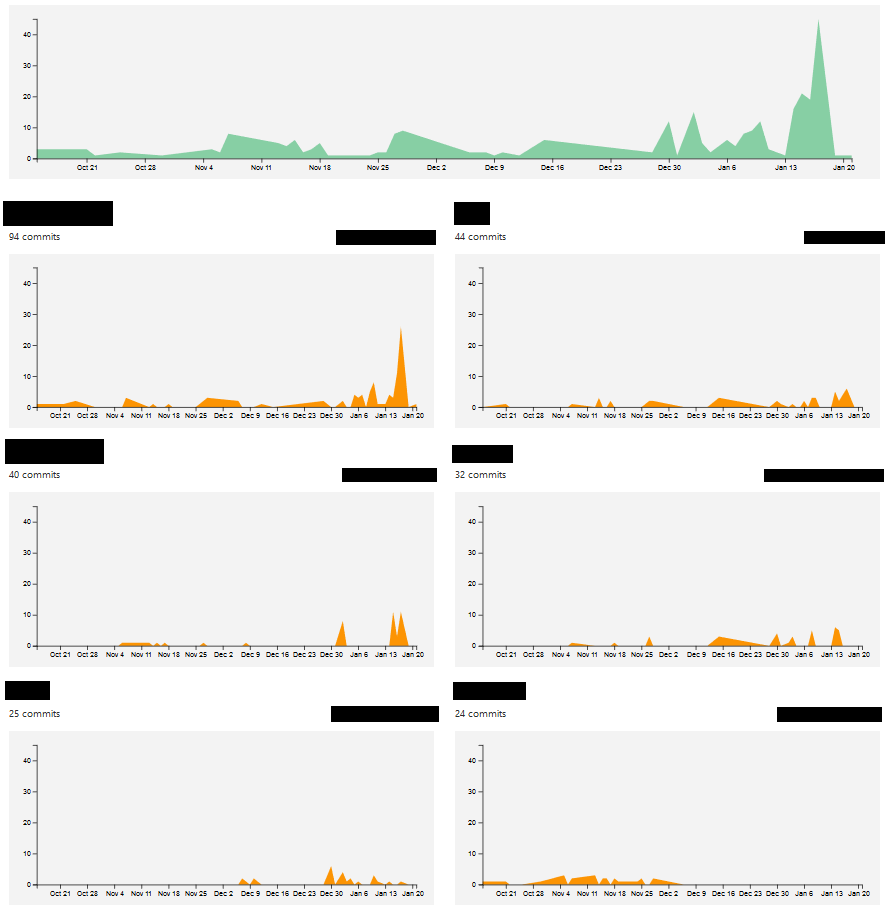
\includegraphics[scale=0.4]{slike/aktivnost.PNG} %veličina slike u odnosu na originalnu datoteku i pozicija slike
			\centering
			\caption{Primjer slike s potpisom}
			\label{fig:promjene}
		\end{figure}
		
		\begin{figure}[H]
			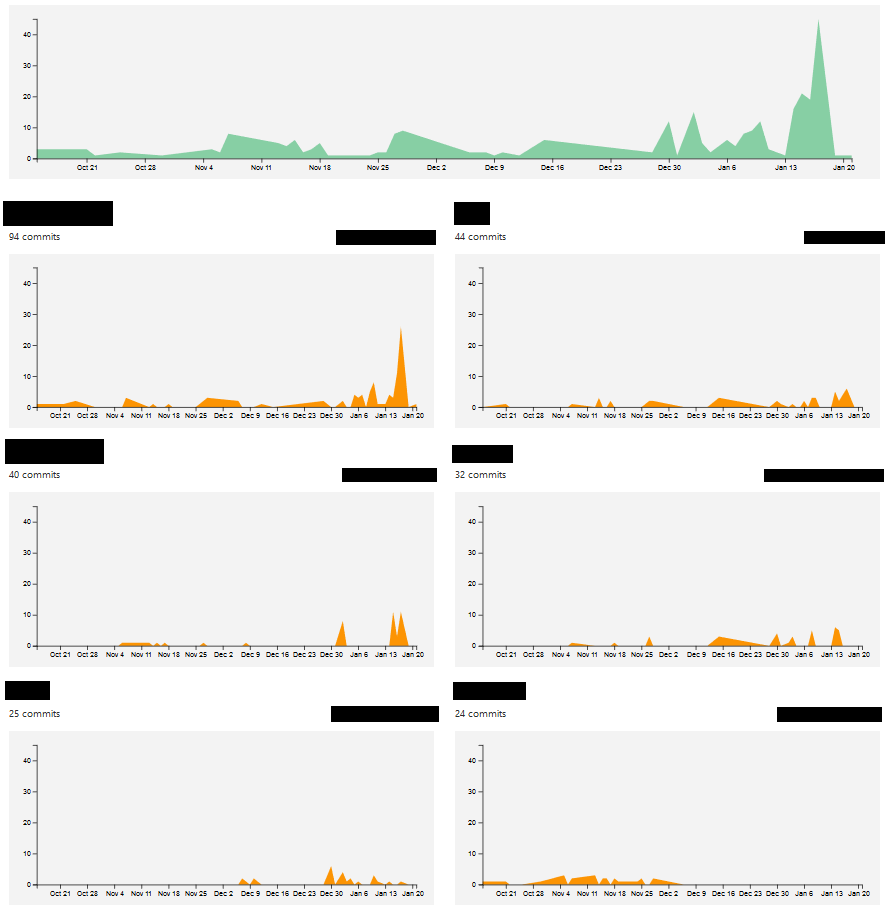
\includegraphics[width=\textwidth]{slike/aktivnost.PNG} %veličina u odnosu na širinu linije
			\caption{Primjer slike s potpisom 2}
			\label{fig:promjene2} %label mora biti drugaciji za svaku sliku
		\end{figure}
		
		Referenciranje slike \ref{fig:promjene2} u tekstu.
		
		\eject
		
	